\subsection{Change}
\label{sec:Suggestion:Change}

\begin{figure}[t]
    \centering
    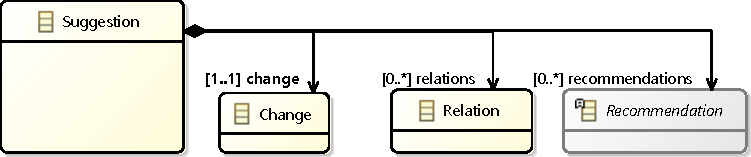
\includegraphics[width=\columnwidth]{images/Suggestion.pdf}
    %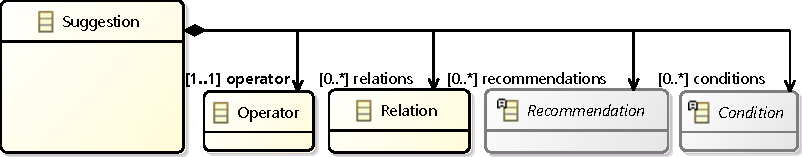
\includegraphics[width=\columnwidth]{images/SuggestionWithCondition.pdf}
    \caption{A \textsf{Suggestion} holds for a single \textsf{Change} linked to 
		elements in a View Type through \textsf{Relation}s, and consists of a set of \textsf{Recommendation}s 
		\HM{add condition element?}\MA{Version WITH \textsf{Condition} is commented in file: switch if needed}.}
    \label{fig:Suggestion}
\end{figure}

\textsf{Operator}s, as shown in Figure~\ref{fig:Operator}, are split into two categories:
\textsf{Primitive} ones operate a single change in \textsf{MM}; while
\textsf{Complex} ones combine several \textsf{Primitive} \textsf{Operator}s
to perform a meaningful change. 
Each \textsf{Operator} may target \emph{any} instantiable \metamodel element, 
thus referring to the meta-class \textsf{NamedElement} and its container, which has same type.

We identified the MM change \textsf{Operator}s based on the work of Herrmannsdoerfer et al.~\cite{herrmannsdoerfer_extensive_2011} who presented a list of 27 primitive and 34 complex operators. In this work, we choose all of the primitive and 7 complex operators, which according to Khelladi et al.~\cite{khelladi_detecting_2015} constitute 72\% of all complex changes appearing in a large case study. 

% HM commented
% Since \viewtypes are structurally \metamodels, we reviewed the literature to
% identify relevant change \textsf{Operator}s for \metamodels and 
% \metamodel{}-model co-evolution. 
% We therefore integrate all 27 \textsf{Primitive} and seven of the 34 
% \textsf{Complex} \textsf{Operator}s in the catalogue proposed by 
% \textcite{herrmannsdoerfer_extensive_2011}.
% Those were selected because according to \textcite{khelladi_detecting_2015}, 
% they constitute 72\% of all complex changes appearing in a large case study. 

\textsf{Operator}s are enriched with \emph{severity}: \textsf{MAJOR}, 
\textsf{MINOR} and \textsf{IGNORE}. 
When applied to a \metamodel, the \textsf{Operator}s in \textsf{IGNORE} have no 
effect on the corresponding \viewtypes; \textsf{Operator}s that can break the 
relationship between \textsf{MM} and its \viewtypes are categorised as \textsf{MAJOR}; 
the rest of the \textsf{Operator}s are \textsf{MINOR}, since they are not 
breaking but can enrich the \viewtypes with additional information.

\begin{figure}[t]
    \centering
    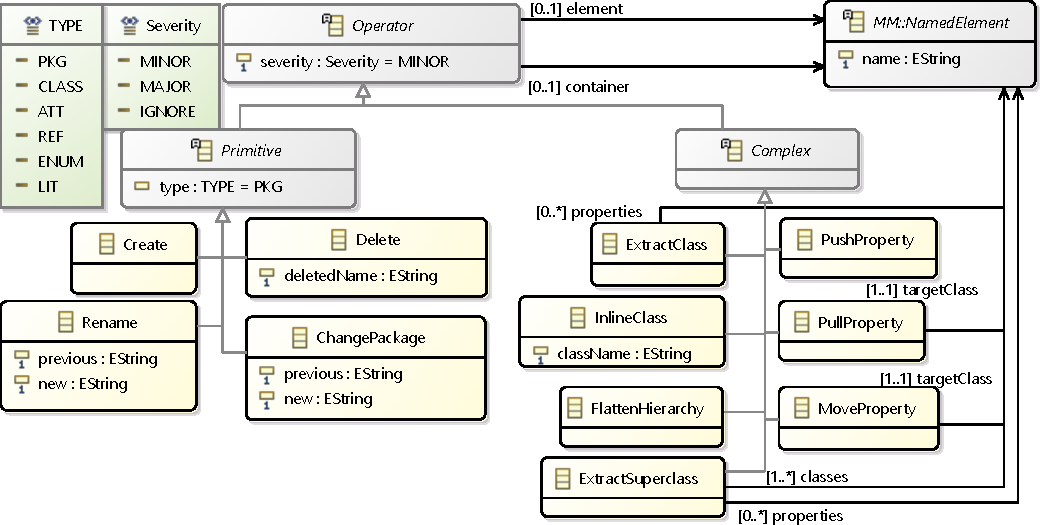
\includegraphics[width=\columnwidth]{Change.pdf}
    \caption{Possible \textsf{Operator}s for \metamodel evolution.}
    \label{fig:Operator}
\end{figure}

Back to our example, the evolution steps of Figure \ref{fig:FSM} make use of different \textsf{Operator}s.
\begin{itemize}
	\item In Step 1 (depicted from Figure \ref{fig:FSM:Init} to \ref{fig:FSM:Relevant}),
	the following sequence of \textsf{Operator}s is applied:
	$$\langle \mathsf{PushProperty} \cdot \mathsf{Rename} \cdot \mathsf{Rename} \rangle$$
	First, \textsf{PushProperty} pushes down $\mathsf{Named} \squaredots \mathsf{name}$
	(i.e. pushes down the \textsf{element} \textsf{name} in the \textsf{container}
	\textsf{Named})
	into each subclass (namely, \textsf{FSM}, \textsf{State} and \textsf{Transition});
	then \textsf{Rename} is applied to the \textsf{ATT}ribute \textsf{element} 
	\textsf{name}, located respectively in \textsf{container}s $\mathsf{FSM}$ and 
	$\mathsf{Transition}$, thus obtaining the result of Figure \ref{fig:FSM:Relevant}.
	
	\item Step 2 only consists of the following \textsf{Operator} sequence:
	$$\langle \mathsf{Create} \cdot \mathsf{Create} \cdot \mathsf{Create} \cdot \mathsf{Create} \rangle$$
	where three of these \textsf{Operator}s add a new \textsf{ATT}ribute \textsf{element}
	in \textsf{container} \textsf{Transition}, and the last one adds a new 
	\textsf{LIT}eral \textsf{element} in the \textsf{container} enumeration \textsf{Kind},
	resulting in the situation of \autoref{fig:FSM:Guard}.
	
	\item Step 3 requires a longer sequence of \textsf{Operator}s, since it creates
	a new class hieararchy under \textsf{Expression}. However, this sequence may
	start with the following:
	$$\langle \mathsf{Delete}^3 \cdot \mathsf{Create}^2 \cdot \ldots \rangle$$
	The initial \textsf{Delete}s undo the three \textsf{Create} \textsf{Operators}s 
	of Step 2
	(thus, referring to the same \textsf{element}s and \textsf{container}); and
	the two following \textsf{Create}s create the new \textsf{Expression} class
	(with the default package as a \textsf{container}) and the \textsf{guard}
	reference (with \textsf{Transition} as a \textsf{container}).
\end{itemize}
With these examples, we immediately notice that some \textsf{Operator}s
in a change sequence may depend on previous ones (e.g. \textsf{Rename}
in Step 1 should only be performed after \textsf{PushProperty}); while others
may freely commute (e.g. the \textsf{Create} in Step 2 may be performed in any 
order).